% By default, the contents of the back side of the final sheet is
% printed upside down. The option notumble suppresses that. Doing so
% may be necessary to suit the behavior of certain printing engines.
% Specifying [notumble] may also be useful during the writing of a
% document, to enable proof-reading on the screen.
\documentclass[notumble]{leaflet}
%\documentclass{leaflet}

\usepackage[utf8]{inputenc}
\usepackage[T1]{fontenc}
\usepackage{lmodern}
\renewcommand{\rmdefault}{iwonac}
\renewcommand{\bfdefault}{b}
\usepackage{microtype}
\usepackage[english,@@LANG@@]{babel}
\usepackage{color, graphicx}
\usepackage{alltt}
\usepackage{url}
\usepackage{ifthen}
\usepackage{xspace}

\newenvironment{stGlossary}
{
\section{\stGlossaryTerm}
\begin{description}
}
{
\end{description}
}

\newcommand{\stWordDefinition}[1]
{\item[\csname st#1Term\endcsname]: \csname st#1Definition\endcsname
}


\newcommand{\stNilTerm}{nil}
\newcommand{\stTrueAndFalseTerm}{true {\rm \stAndTerm} false}
\newcommand{\stSelfTerm}{self}
\newcommand{\stSuperTerm}{super}
\newcommand{\stThisContextTerm}{thisContext}


% Change that to english, german or french
\input{@@LANG@@} %%

\makeatletter
\newsavebox{\code@box}
\definecolor{light-gray}{rgb}{0.9,0.9,0.9}
\newenvironment{displaycode}{%
	\begin{lrbox}{\code@box}%
		\begin{minipage}{\linewidth}
			\begin{alltt}\small
}{
			\end{alltt}
		\end{minipage}
	\end{lrbox}
	\colorbox{light-gray}{\usebox{\code@box}}
}
%\let\code\texttt
% Use of english prevents babel from adding spaces before $:
\newcommand{\code}[1]{\foreignlanguage{english}{\texttt{#1}}}
\makeatother

\graphicspath{{figures/}} 

\title{
	\vfill
	\resizebox{\linewidth}{!}{\fontfamily{iwonac}\selectfont Smalltalk}%
	\\[\baselineskip]
	\normalfont
        \stSmalltalkSubtitle
        \\
	\vfill
	
\includegraphics[width=\textwidth]{esug}
}

\date{}
\CutLine*{1} \CutLine*{2} \CutLine*{3} \CutLine*{4} \CutLine*{5}
\CutLine*{6}


% \AddToBackground*{2}{% Background of a large page
%   \put(\LenToUnit{.25\paperwidth},\LenToUnit{.4\paperheight}){%
%     
\includegraphics[width=14.85cm]{esug-background}
% }}

\begin{document}
\maketitle
\thispagestyle{empty}

\pagebreak{}

\section{\stSmalltalkConceptsTerm}

\stSmalltalkConceptsDefinition

\subsection{\stSmalltalkSyntaxTerm}
\paragraph{\stReservedWordsTerm}
\begin{description}
\stWordDefinition{Nil}
\stWordDefinition{TrueAndFalse}
\stWordDefinition{Self}
\stWordDefinition{Super}
\stWordDefinition{ThisContext}
\end{description}

\paragraph{\stReservedCaractersTerm}

\begin{description}
\item[:=] (\stOrTerm $\leftarrow$):  \stAssignmentOperatorDefinition
\item[\^{}] (\stOrTerm $\uparrow$): \stReturnOperatorDefinition
\item[$\mid$ var1 var2 var3 $\mid$]: \stTempsDeclarationOperatorDefinition
\item[\$a]: \stDollarOperatorForCharacterADefinition
\item[\#(abc 123)]: \stLiteralArrayDefinition
\item[.]: \stDotOperatorDefinition
\item[;]: \stSemiColonOperatorDefinition
\item[[ ]]: \stBlockOperatorDefinition
\item["\stCommentTerm"].
\item['\stStringTerm'].
\end{description}

\pagebreak{}

\subsection{\stMessageSendingTerm}

\stMessageSendingDefinition

\paragraph{\stUnaryMessagesTerm}

\stUnaryMessagesDefinition

\paragraph{\stBinaryMessagesTerm}

\stBinaryMessagesDefinition

\paragraph{\stKeywordMessagesTerm}

\stKeywordMessagesDefinition

\pagebreak{}

\section{\stDevelopmentEnvironmentTerm}

\stDevelopmentEnvironmentDefinition

\begin{center}
  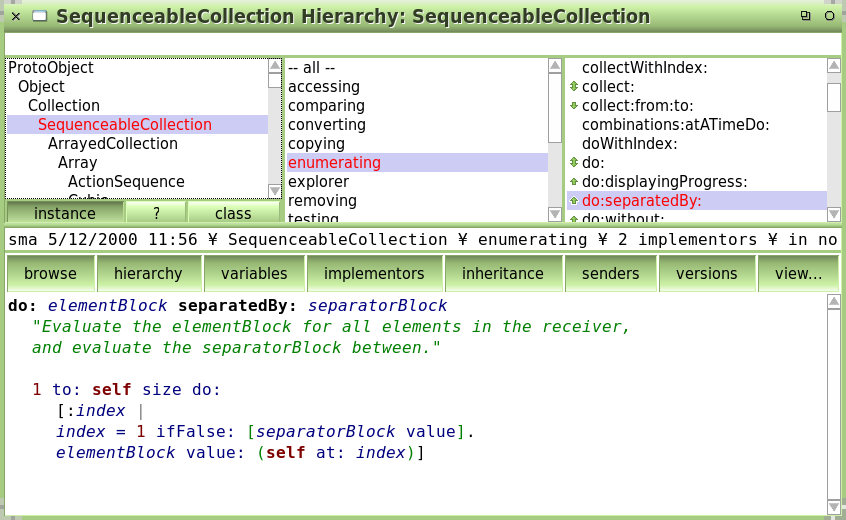
\includegraphics[width=.9\textwidth]{squeak}\\
  \stSqueakCodeBrowserTerm
\end{center}

\section{\stImplementationTerm}

\stImplementationDefinition

\pagebreak{}

\section{\stApplicationsTerm}

\stApplicationsDefinition

\begin{center}
  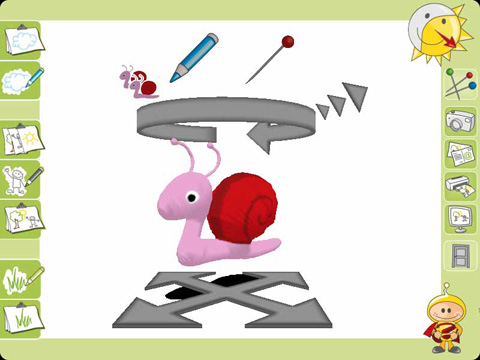
\includegraphics[width=.5\textwidth]{plopp}\\
  \stPloppDrawingSessionTerm
\end{center}

\begin{stGlossary}
\stWordDefinition{Image}
\stWordDefinition{VM}
\stWordDefinition{Reflexion}
\stWordDefinition{DynamicTyping}
\end{stGlossary}

\pagebreak{}

\section{\stBooksTerm}

\stBooksDefinition

\section{\stSmalltalkActionsTerm}

\stSmalltalkActionsDefinition

\section{Internet}

\stInternetWebsitesDefinition

\end{document}  

%%% Local Variables:
%%% coding: utf-8-unix
%%% mode: latex
%%% TeX-master: t
%%% TeX-PDF-mode: t
%%% ispell-local-dictionary: "francais"
%%% End:
